% Q4: regular hexagon from the fixed candidate PDF, printed page 334.
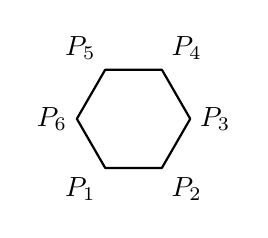
\begin{tikzpicture}[line cap=round,line join=round,x=0.72cm,y=0.72cm]
  \coordinate (P1) at (0,0);
  \coordinate (P2) at (1,0);
  \coordinate (P3) at (1.5,0.866);
  \coordinate (P4) at (1,1.732);
  \coordinate (P5) at (0,1.732);
  \coordinate (P6) at (-0.5,0.866);
  \draw[thick] (P1)--(P2)--(P3)--(P4)--(P5)--(P6)--cycle;
  \node[below left] at (P1) {$P_1$};
  \node[below right] at (P2) {$P_2$};
  \node[right] at (P3) {$P_3$};
  \node[above right] at (P4) {$P_4$};
  \node[above left] at (P5) {$P_5$};
  \node[left] at (P6) {$P_6$};
\end{tikzpicture}
